\documentclass[12pt,a4paper]{article}

\usepackage[T1]{fontenc}
\usepackage[utf8]{inputenc}
\usepackage[english]{babel}
\usepackage{amsmath}
% Fonts: Libertinus for text and maths, Inconsolata for code
\usepackage[tabular,lining]{libertinus-type1}
\usepackage{libertinust1math}
\usepackage[varqu,varl,scaled=0.95]{zi4}
\usepackage{microtype}
\usepackage[margin=2.5cm, headheight=15pt, headsep=18pt, footskip=28pt]{geometry}
\usepackage{xcolor}
\definecolor{accent}{RGB}{28,63,110}
\usepackage{booktabs}
\usepackage{longtable}
\usepackage[skip=6pt, font=small, labelfont={sf,bf,color=accent}]{caption}
\usepackage{float}
\usepackage{array}
\usepackage{enumitem}
\usepackage{verbatim}
\usepackage[obeyspaces]{url}
\usepackage{pgfplots}
\pgfplotsset{compat=1.17}
\usepackage{titlesec}
\usepackage{fancyhdr}
\usepackage{etoolbox}
\usepackage{needspace}
\usepackage{tcolorbox}
\usepackage[colorlinks=true, allcolors=accent,
  pdftitle={Improving the SBAM implementation in the SMILE model}]{hyperref}

\setlist{itemsep=2pt, topsep=4pt}
\setlength{\parindent}{0pt}
\setlength{\parskip}{6pt}
\setlength{\emergencystretch}{2em}
\renewcommand{\arraystretch}{1.15}

\newcommand{\kode}[1]{\texttt{#1}}

% Let tables and figures stay close to the text that refers to them
\renewcommand{\topfraction}{0.9}
\renewcommand{\bottomfraction}{0.7}
\renewcommand{\textfraction}{0.08}
\renewcommand{\floatpagefraction}{0.8}
\setcounter{topnumber}{3}
\setcounter{bottomnumber}{2}
\setcounter{totalnumber}{4}

% Headings
\titleformat{\section}{\sffamily\bfseries\Large\color{accent}}{\thesection}{0.7em}{}
\titleformat{\subsection}{\sffamily\bfseries\large\color{accent}}{\thesubsection}{0.7em}{}
\titleformat{\subsubsection}{\sffamily\bfseries\normalsize}{\thesubsubsection}{0.7em}{}
\titlespacing*{\section}{0pt}{20pt plus 4pt minus 2pt}{6pt plus 1pt}
\titlespacing*{\subsection}{0pt}{14pt plus 3pt minus 2pt}{3pt plus 1pt}
\titlespacing*{\subsubsection}{0pt}{10pt plus 2pt minus 1pt}{1pt plus 1pt}

% Header and footer
\pagestyle{fancy}
\fancyhf{}
\renewcommand{\sectionmark}[1]{\markboth{\thesection\quad #1}{}}
\renewcommand{\subsectionmark}[1]{}
\fancyhead[L]{\small\sffamily\color{black!55}Improving the SBAM implementation in the SMILE model}
\fancyhead[R]{\small\sffamily\color{black!55}\leftmark}
\fancyfoot[C]{\small\sffamily\color{black!70}\thepage}
\renewcommand{\headrulewidth}{0.4pt}
\renewcommand{\headrule}{{\color{black!25}\hrule width\headwidth height\headrulewidth}\vskip-\headrulewidth}
\fancypagestyle{plain}{\fancyhf{}\fancyfoot[C]{\small\sffamily\color{black!70}\thepage}%
  \renewcommand{\headrulewidth}{0pt}}

% Code blocks on a light grey background
\tcbuselibrary{breakable}
\BeforeBeginEnvironment{verbatim}{\begin{tcolorbox}[breakable, lines before break=4, colback=black!4, colframe=black!4, boxrule=0pt,
  arc=2pt, left=6pt, right=6pt, top=1pt, bottom=1pt, boxsep=3pt, fontupper=\small,
  before skip=9pt, after skip=11pt]}
\AfterEndEnvironment{verbatim}{\end{tcolorbox}}

\begin{document}
\thispagestyle{plain}

{\raggedright
{\sffamily\bfseries\LARGE\color{accent}Improving the SBAM implementation\\ in the SMILE model\par}
\vspace{6pt}
{\sffamily\large\color{black!70}A test on an artificial marriage market\par}
\vspace{10pt}
{\color{accent}\hrule height 1.2pt}
\vspace{8pt}
{\sffamily\small\color{black!60}21 November 2026\par}
}
\vspace{1.4em}

{\sffamily\bfseries\color{accent}Abstract\par}
\vspace{-2pt}
{\small
SBAM is the algorithm that decides who forms a couple with whom in SMILE, DREAM's microsimulation
model of the Danish population. This paper tests the implementation of SBAM in the model's code. The
model can only be run on DREAM's closed server at Statistics Denmark, so the code is run in a small
stand-alone program on an artificial marriage market, built on Choo and Siow's (2006) model, where
the correct answer is known. The code forms the right number of couples, but it pairs too many
people who do not resemble each other. With the model's scale-up of the pool, 61.5 per cent of the
couples are from the same region and 46.8 per cent have the same education, against 76.7 and 55.4
per cent in the correct answer. The bias arises in the last step, where the computed couple table
is turned into couples, and from the model's second year the code no longer uses the historical
table. The paper then tries out five changes to the code. It ends with a method that is both more
precise and faster than the existing code: the method hits the correct answer, and a call of the
matching takes 16--36 ms in all the cases tested, against 26--965 ms for the existing code.\par}
\vspace{4pt}
{\color{black!25}\hrule height 0.4pt}
\vspace{0.4em}

\section{Introduction}

SMILE is DREAM's microsimulation model, which projects the Danish population person by person. Each
year the model selects the singles who are to form couples, and an algorithm decides who forms a
couple with whom. The algorithm is called SBAM and is described by Stephensen and Markeprand (2013).
The code is in the file \kode{Matching.cs}. This paper tests whether the code does what SBAM is
supposed to do.

The model cannot be run outside DREAM's closed server at Statistics Denmark, because its data are
not available there. The code has therefore been lifted out into a small stand-alone program and run
on an artificial marriage market. The market is constructed so that it is known how many couples are
formed on average between each type of man and each type of woman. The couples formed by the code
can therefore be compared with the correct answer. The algorithm in the code itself has not been
changed.

The test gives four results:

\begin{enumerate}
\item \textbf{The code forms the right number of couples.} It forms 36,132 of the 36,332 couples it
is supposed to form (99.45 per cent), and all 36,293 in the run with the model's scale-up. No person
is in more than one couple, and every couple consists of a man and a woman.

\item \textbf{The code pairs too many people who do not resemble each other.} On the artificial
market the man and the woman live in the same region in 76.7 per cent of the couples, and they have
the same education in 55.4 per cent. A correct SBAM hits both figures. Among the couples formed by
the code, the shares are only 67.0 and 49.8 per cent (Figure~\ref{fig:sortering}). The deviation is
many times larger than chance can explain.

\item \textbf{It gets worse with the model's scale-up.} SMILE selects more people to form couples
than are needed and stops when the number of couples has been reached. With the model's factor of
1.3 the shares fall to 61.5 and 46.8 per cent.

\item \textbf{The error is in the last step, where the couples are formed.} SBAM first computes a
table of how many couples of each kind are to be formed and then forms the couples. The table is
almost right, even though the computation stops too early because of a programming error. The bias
arises when the table is turned into couples. The probable cause is that rare combinations are
allowed to draw lots for a couple many times. That agrees with the code's own counters and has been
confirmed by correcting the code in a copy (Section~\ref{sec:nymetode}).
\end{enumerate}

\begin{figure}[htb]
\centering
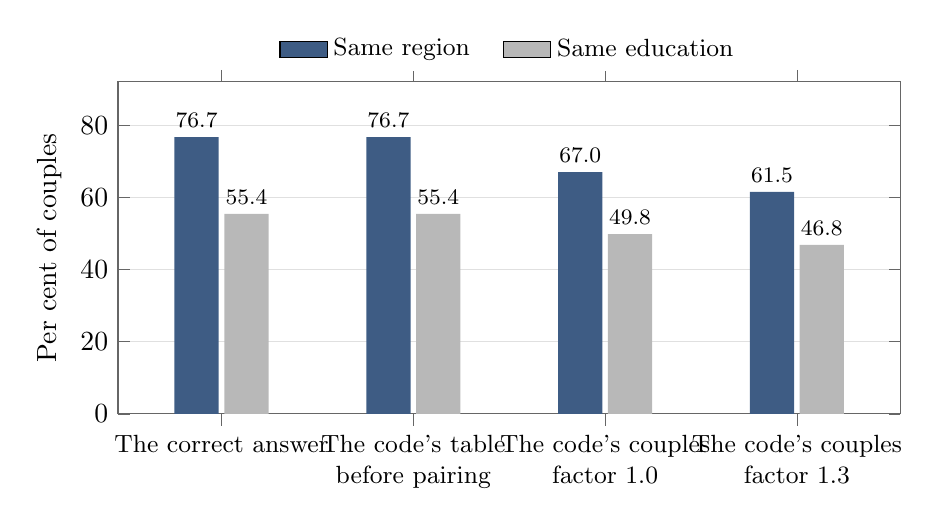
\begin{tikzpicture}
\begin{axis}[
  ybar, area legend, bar width=16pt, width=0.95\textwidth, height=5.8cm,
  ymin=0, ymax=92, enlarge x limits=0.18,
  ylabel={Per cent of couples},
  symbolic x coords={a,b,c,d}, xtick=data,
  xticklabels={{The correct answer},{The code's table\\before pairing},{The code's couples\\factor 1.0},{The code's couples\\factor 1.3}},
  x tick label style={align=center, font=\small},
  ymajorgrids, grid style={black!12}, axis line style={black!60}, tick style={black!60},
  nodes near coords,
  nodes near coords style={font=\footnotesize, /pgf/number format/.cd, fixed, fixed zerofill, precision=1},
  legend style={at={(0.5,1.03)}, anchor=south, legend columns=2, draw=none, font=\small, /tikz/every even column/.append style={column sep=1em}},
]
\addplot[fill=accent!85, draw=none] coordinates {(a,76.7) (b,76.7) (c,67.0) (d,61.5)};
\addplot[fill=black!28, draw=none] coordinates {(a,55.4) (b,55.4) (c,49.8) (d,46.8)};
\legend{Same region, Same education}
\end{axis}
\end{tikzpicture}
\caption{Share of couples in which the man and the woman live in the same region and have the same
education. The code's table before pairing has been recomputed in the test and has the same shares
for both factors. The factor is the model's scale-up of the pool; 1.0 means no scale-up.}
\label{fig:sortering}
\end{figure}

The paper then tries out five changes to the code. Four of them correct the method, and the fifth
computes the same table faster. They are made in a copy, \kode{Matching\_test.cs}, and are described
in Section~\ref{sec:nymetode}. This gives three more results:

\begin{enumerate}[resume]
\item \textbf{From the model's second year the code does not use the historical table.} When the
table is reset after a year's matching, all cells get the value 1. After that only 43.7 per cent of
the couples are from the same region and 41.4 per cent have the same education. The error has been
read in the code and demonstrated in the test. How much it matters in the model depends on the
model's data.

\item \textbf{With the changes the code hits the correct answer.} 76.7 per cent of the couples are
from the same region, and 55.4 per cent have the same education. 1.8 per cent of the couples are
misplaced relative to a correct SBAM, against 24.8 per cent before. This also holds in a small pool,
in a pool with fewer men than women and in a pool with a different composition from the historical
data.

\item \textbf{With all five changes the code is also faster.} The first four changes alone make the
code slower in the typical case: with factor 1.3 one year's matching takes 74 ms on the test market
against 44--46 ms before. Most of the time goes to computing the table. The fifth change computes
the same table at least 20 times faster. One year's matching then takes 32 ms with factor 1.3 and
26 ms without scale-up, where \kode{Matching.cs} uses about 810 ms.
\end{enumerate}

The test does not cover everything. Among other things, it does not touch a possible error in the
code's age indexing and says nothing about types of persons that are not found in the historical
data (Section~\ref{sec:forbehold}).


\section{Background: what SBAM does}\label{sec:sbam}

\subsection{The task}

A microsimulation model has to form new couples every year. This happens in two steps. First, the
singles who are to find a partner during the year are selected; they make up the \emph{pool}. Then
the men and women in the pool have to be put together two by two. The second step is called
matching, and that is what this paper is about.

The matching has to reproduce the fact that couples are not formed at random. Partners typically
resemble each other in age and education and live near each other. The pattern of who forms a couple
with whom is called the \emph{sorting} in this paper.

The persons are divided into \emph{types}. A type is a combination of characteristics, for example
a 30-year-old man with a vocational education living in East Jutland. The sorting can then be
written as a \emph{couple table} with a row for each type of man and a column for each type of
woman. Each entry in the table, a \emph{cell}, contains the number of couples of exactly that
combination.

\subsection{The algorithm in three steps}

SBAM (Sparse Biproportionate Adjustment Matching) builds on a couple table from historical data.

\begin{enumerate}
\item \textbf{Historical table.} The couples formed over a number of years are counted in a couple
table $X^0$. The table shows the historical pattern but does not fit this year's pool, which has a
different size and composition.

\item \textbf{Adjustment to the pool (RAS).} The table is adjusted so that the sum of each row
equals the number of men of that type in the pool, and the sum of each column equals the number of
women. This is done by alternately multiplying each row and each column by a factor until the sums
match. The method is called RAS or biproportional adjustment. One scaling of all rows and one of
all columns is called a \emph{pass} here. The adjustment preserves the pattern of the historical
table as well as the pool allows.

\item \textbf{Pairing.} For each cell in the adjusted table, as many couples as the cell states are
drawn at random among the pool's men and women of the two types. The cells do not normally contain
whole numbers, so rounding is needed. It can be done by drawing lots: a cell with the value 2.3
gives two couples and, with probability 0.3, a third.
\end{enumerate}

An example with two types of each sex shows step 2. Historically 200 couples were formed, most of
them between like types. This year's pool has 60 men of type 1 and 40 of type 2, and 50 women of
each type:

\begin{center}
\begin{tabular}{@{}lrrcrrr@{}}
\toprule
 & \multicolumn{2}{c}{Historical table $X^0$} & & \multicolumn{3}{c}{Adjusted to the pool} \\
\cmidrule(lr){2-3}\cmidrule(l){5-7}
 & Woman 1 & Woman 2 & & Woman 1 & Woman 2 & Men in the pool \\
\midrule
Man 1 & 80 & 20 & & 44.1 & 15.9 & 60 \\
Man 2 & 20 & 80 & & 5.9 & 34.1 & 40 \\
\midrule
Women in the pool & & & & 50 & 50 & \\
\bottomrule
\end{tabular}
\end{center}

The adjusted table uses everyone in the pool, and couples between like types are still by far the
most frequent. In step 3 the top-left cell gives 44 couples and, with probability 0.1, one more.

\subsection{What is special about the code in SMILE}

Four features of \kode{Matching.cs} matter for the test:

\begin{itemize}
\item \textbf{Many types.} A type is a combination of sex, age (15--65), education (5 levels),
residence (11 provinces or 98 municipalities) and origin (5 groups). That gives 28,050 types with
provinces and 249,900 with municipalities.

\item \textbf{Men and women are in the same table.} The code has one list of types, in which sex is
part of the type. A couple is therefore counted in two cells that are mirror images of each other.
Before the pairing the two cells are added together, so a cell's value in the code is twice the
number of couples the cell is to give.

\item \textbf{The pool is larger than necessary.} The model multiplies the probability of entering
the pool by a factor, \kode{MatchingScaleUp}, which is between 1.05 and 1.3 depending on
municipality. The code then forms only as many couples as correspond to the size of the pool divided
by the factor, and stops. With factor 1.3, about 23 per cent of the pool thus remain without a
partner. The surplus is there to ensure that the number of couples can be reached.

\item \textbf{The pairing takes place in several passes.} The code goes through the cells up to 1000
times and takes at most one couple from the integer part of a cell each time. This is described in
more detail in Section~\ref{sec:fortolkning}.
\end{itemize}

\subsection{Terms used in the paper}

\begin{longtable}{@{}lp{11.3cm}@{}}
\toprule
Term & Meaning \\
\midrule
\endhead
Type & A combination of characteristics of a person: age, education, residence and, in SMILE, also origin. \\
Pool & The singles who are selected in a year to form couples. \\
Couple table & The number of couples for each combination of the man's and the woman's type. \\
Cell & One entry in the couple table. \\
Sorting & The pattern of who forms a couple with whom, that is, the distribution of couples over cells. \\
RAS & Alternate scaling of rows and columns until the sums of the table match the pool. \\
Pass & In RAS, one scaling of all rows and all columns. In the pairing, one trip through all cells. \\
Factor & The model's scale-up of the pool, \kode{MatchingScaleUp}. Factor 1.0 is no scale-up. \\
Seed & Starting value for the random numbers. The same seed gives the same run. \\
\bottomrule
\end{longtable}
\addtocounter{table}{-1}% the list of terms is not a numbered table


\section{Set-up of the test}\label{sec:opstilling}

\subsection{The idea}

On real data one cannot decide whether a matching algorithm gets it right, because the true pattern
is not known. The test therefore uses an artificial market where it is. The market is built on
Choo and Siow's (2006) model of the marriage market. The test has five steps:

\begin{enumerate}
\item A market is set up with single men and women and a \emph{true couple table} $\mu$, which
states how many couples are formed on average in a year in each cell.
\item From the true table, five years of ``register data'' are drawn: the couples that happened to
be formed in each of the years. These are the historical data the code receives.
\item A pool of singles who are to form couples is selected.
\item \kode{Matching.cs} reads the historical data and forms couples from the pool.
\item The couples formed are compared with the true table and with what a correct SBAM would give.
\end{enumerate}

\subsection{The artificial market}

The market is constructed for the test. Everything needed to understand the test is stated here.
Appendix~\ref{app:parametre} describes the market in full, with all parameter values and the
method of computation, so that it can be reproduced.

\textbf{Types and population.} A type is a combination of age (20--54 in one-year steps), education
(3 levels) and region (4 regions). That gives 420 types for each sex and $420\times420=176{,}400$
cells in the couple table. There are 299,997 single men and 300,003 single women. The young are the
most numerous, the women are on average better educated than the men, and region~1 is the largest
and the best educated.

\textbf{The true couple table.} The table is computed with Choo and Siow's (2006) model. In the
model the number of couples between men of type $x$ and women of type $y$
depends on two things: how many singles there are of the two types, and how large a gain
$\Phi_{xy}$ the two have from forming a couple rather than remaining single:
\[
\mu_{xy}=\sqrt{\mu_{x0}\,\mu_{0y}}\;\exp(\Phi_{xy}/2) .
\]
Here $\mu_{x0}$ and $\mu_{0y}$ are the numbers of men and women of the two types who remain single.
All singles either form a couple or remain single, so
$\mu_{x0}+\sum_y\mu_{xy}=M^A_x$ and $\mu_{0y}+\sum_x\mu_{xy}=M^B_y$, where $M^A_x$ and $M^B_y$ are
the numbers of single men and women of each type. The equations have exactly one solution for a
given population (Decker et al., 2013). It has been found with the iterative method of Galichon and
Salanié (2022), which is described in Appendix~\ref{app:parametre}.

The gain is chosen so that the pattern has the features known from real couples:
\[
\frac{\Phi_{xy}}{2}=\kappa+h_A(a_x)+h_B(a_y)-\frac{(a_x-a_y-2)^2}{2\,\tau(\bar a_{xy})^2}
+\rho^E_{e_xe_y}+\rho^R_{r_xr_y},
\]
where $a$, $e$ and $r$ are age, education and region. The terms mean:

\begin{itemize}
\item $h_A$ and $h_B$: the gain from forming a couple falls with age for both sexes, so the young
form couples more often than the old.
\item The quadratic term: the preferred age gap is that the man is two years older. The tolerance
$\tau$ for deviations grows with the couple's mean age $\bar a_{xy}$ from 2 to 6 years.
\item $\rho^E$: couples with the same education have an extra gain, and couples with the lowest and
the highest education have a penalty.
\item $\rho^R$: couples across regions have a large penalty, though a smaller one for the two
neighbouring regions 1 and 2.
\item $\kappa$: a constant that is set so that 12 per cent of the single men find a partner in a
year.
\end{itemize}

Table~\ref{tab:marked} shows the resulting market. The figures are not meant to resemble a
particular country, but the orders of magnitude are realistic. The share of singles of a type who
form a couple in a year is called the \emph{match rate} of the type.

\begin{table}[htb]
\centering
\caption{The artificial market. An extreme couple has an age gap that is more than 10 years from
the typical gap of 2 years.}
\label{tab:marked}
\begin{tabular}{@{}lr@{}}
\toprule
Single men & 299,997 \\
Single women & 300,003 \\
New couples per year & 36,000 \\
Age gap, mean (the man's age minus the woman's, years) & 1.88 \\
Age gap, standard deviation (years) & 3.28 \\
Couples with the same education (per cent) & 55.4 \\
Couples from the same region (per cent) & 76.7 \\
Extreme couples (per cent) & 0.53 \\
Match rate for men aged 25 (per cent) & 17.55 \\
Match rate for men aged 50 (per cent) & 5.80 \\
\bottomrule
\end{tabular}
\end{table}

\textbf{Why the market is a fair test of SBAM.} In Choo and Siow's model the true table has the form
$\mu_{xy}=\alpha_x\beta_yK_{xy}$, where $K=\exp(\Phi/2)$ is fixed, and $\alpha$ and $\beta$ depend
on the population. The true table for another population is therefore a biproportional adjustment
of the true table for the first one. That is exactly the assumption SBAM builds on. A correct SBAM
should thus be able to reproduce the sorting on this market, apart from the noise in the historical
data and the noise that comes from rounding. If the code deviates by more than that, it is the
fault of the code and not of the method.

\subsection{Historical data}

Real register data are not the true table but one random outcome of it. This is imitated by drawing
the number of couples in each cell from a Poisson distribution with mean $\mu_{xy}$, independently
for each cell and each year. Five years are drawn, and the sum is called $X^0$. It contains 180,627
couples spread over 36,454 of the 176,400 cells; the rest are empty.

The couples are written to a text file in the format \kode{Matching.cs} reads, with one line for
each person in each couple.

\subsection{The pool}

In SMILE it is other parts of the model that determine who enters the pool. In the test this is
imitated as follows: each single enters the pool with a probability equal to the share of his or
her type that formed a couple per year in the historical data. Men and women are drawn
independently, so the numbers of each sex are not exactly equal. The larger side is therefore cut
down at random to the size of the smaller. The numbers of men and women of each type in the pool
are called $n^A_x$ and $n^B_y$.

With a factor $s$ above 1 the probability of entering the pool is multiplied by $s$, as the model
does. The pool then becomes $s$ times larger, and the code forms couples from only about $1/s$ of
it.

\subsection{How the market is embedded in SMILE's types}\label{sec:indlejring}

The code works with SMILE's 28,050 types, while the market has 840 (420 for each sex). The market's
types have therefore been translated into SMILE's:

\begin{center}
\begin{tabular}{@{}lp{0.66\textwidth}@{}}
\toprule
The market & SMILE \\
\midrule
Age 20--54 & The same age \\
Education 1, 2, 3 & Primary and lower secondary school, vocational education and long-cycle higher education \\
Region 1, 2, 3, 4 & The provinces City of Copenhagen, Copenhagen surroundings, Funen and East Jutland \\
 & The municipalities of Copenhagen, Gentofte, Odense and Aarhus \\
Origin & Danish origin for all \\
Years of the historical data & 2008--2012, which are the years the code selects \\
\bottomrule
\end{tabular}
\end{center}

Two choices in the translation matter for what the test measures:

\begin{itemize}
\item \textbf{The age in the data file is set one year down.} The code adds 1 to the age when it
reads the historical data, because the model's data measure age at the beginning of the year, while
the matching takes place at the end of the year. The data file is made so that the historical
couples and the pool end up in the same types.
\item \textbf{All types in the pool are found in the historical data.} A type without historical
couples has match rate 0 and never enters the pool.
\end{itemize}

\subsection{What the code's couples are compared with}

The couples formed by the code are counted in a couple table $T$. It is compared with four other
tables:

\begin{description}[leftmargin=1.5em, style=nextline]
\item[True model] The true table $\mu$. This is the correct answer.
\item[True model, one draw] One random outcome of the true table, drawn in the same way as one year
of the historical data. Even a perfect algorithm does not hit $\mu$ exactly in a single run,
because the number of couples in a cell is random. This table shows how large a deviation that
gives.
\item[Reference SBAM] SBAM carried out correctly: the historical table $X^0$ adjusted to the pool
with RAS until the sums match. It is the adjusted table itself, that is, before rounding to whole
couples.
\item[The code's RAS table] The table the code arrives at when its RAS stops after two passes
(Section~\ref{sec:ras}). The table has been recomputed in the test program by the same procedure as
the code; it has not been read from inside the code.
\end{description}

The comparison uses two kinds of measures. The first is simple key figures for the couples: the age
gap and its dispersion, the share of extreme couples and the shares with the same education and the
same region.

The second is an overall measure of how differently two tables distribute the couples. The
dissimilarity index (Duncan and Duncan, 1955) is
\[
D=50\sum_{g,h}\left|\frac{T_{gh}}{T_{\cdot\cdot}}-\frac{\mu_{gh}}{\mu_{\cdot\cdot}}\right| ,
\]
where $T_{gh}/T_{\cdot\cdot}$ is the share of the couples in the table $T$ that lie in cell
$(g,h)$, and $\mu_{gh}/\mu_{\cdot\cdot}$ is the corresponding share in the table it is compared
with. $D$ is the share of the couples, in per cent, that would have to be moved to another cell for
the two distributions to become identical. If $D=10$, every tenth couple is thus misplaced. The
index does not depend on how many couples there are.

The index is computed on four groupings of the types: age in one-year steps ($D_{\text{age}}$),
education ($D_{\text{edu}}$), region ($D_{\text{reg}}$) and a joint grouping by five-year age
groups, education and region ($D_{\text{joint}}$). The finer the grouping, the more room chance
takes up in the index. The code's $D$ should therefore always be held up against the row ``one
draw''.


\section{Results}\label{sec:resultater}

\subsection{The three runs}

Three runs have been made with the same historical data and the same seed
(Table~\ref{tab:koersler}): one without scale-up, one with factor 1.3 and one without scale-up in
which the code divides by municipalities instead of provinces.

\begin{table}[htb]
\centering
\caption{Number of couples in the three runs. The target is the number of couples the code itself
computes that it is to form. The two bottom lines are the code's own counters.}
\label{tab:koersler}
\begin{tabular}{@{}lrrr@{}}
\toprule
 & Factor 1.0 & Factor 1.3 & Factor 1.0 \\
 & provinces & provinces & municipalities \\
\midrule
Persons in the pool & 72,666 & 94,366 & 72,666 \\
Target number of couples & 36,332 & 36,293 & 36,332 \\
Couples formed & 36,132 & 36,293 & 36,132 \\
\quad in per cent of the target & 99.45 & 100.00 & 99.45 \\
Persons without a partner & 402 & 21,780 & 402 \\
\quad in per cent of the pool & 0.55 & 23.08 & 0.55 \\
Passes in RAS & 2 & 2 & 2 \\
Time in the matching (sec.) & 1.0--1.4 & 0.1 & 1.1--1.2 \\
\midrule
Attempts that gave a couple (\kode{succes}) & 36,132 & 36,293 & 36,132 \\
Attempts that lacked a person (\kode{udeladt}) & 22,882 & 5,743 & 22,882 \\
\bottomrule
\end{tabular}
\end{table}

The number of couples is hit in all three runs. The test program also checks four things, all of
which are in order: no household is in more than one couple, all those matched were in the pool, no
couple has the same sex, and the number of couples does not exceed the target.

The run with municipalities forms exactly the same couples as the run with provinces. That is
expected, because the market's four regions correspond one-to-one to four municipalities. The run
therefore only shows that the code also runs with types divided by municipality.

\needspace{12\baselineskip}
\subsection{The RAS adjustment stops too early}\label{sec:ras}

In all three runs the code reports that RAS stopped in the second pass. The cause is an error in
the test that is to decide whether the adjustment is finished (\kode{RASMatrix.cs}, lines 521--527):

{\small
\begin{verbatim}
        err = (r_ssq + c_ssq) / n;
        //if (ConsoleMessage) Console.WriteLine("--> {0}", err);
        double err0 = err;
        if (err < errOK) break;
        if (itt > ittMax) break;
        if (itt > 0 && err - err0 < 0.00001) break;
        itt++;
\end{verbatim}
}

\kode{err} measures how far the sums of the table are from the pool. The second-to-last line is
meant to stop the loop when the error no longer gets smaller from one pass to the next. But
\kode{err0}, which should remember the error from the previous pass, is set equal to the new error
just before the comparison. The difference is therefore always 0, and the loop stops in the second
pass, however large the error is.

The adjustment is not finished at that point. The sums deviate by a total of 2,103 persons out of
72,666, measured during the second pass, and a correct RAS needs 61 passes on the same data.

The consequence for the sorting is nevertheless small on this market. The table after two passes
has the same share of couples with the same education and region as the finished one and deviates
0.9 per cent from it, measured by $D_{\text{joint}}$ (Table~\ref{tab:mod_reference}). This holds
when the pool resembles the population the historical data come from, as it does here. The test
says nothing about a pool that deviates more.

\subsection{The sorting without scale-up}

Table~\ref{tab:sortering10} shows the sorting in the run with factor 1.0. The four top rows are
close to each other: the reference SBAM and the code's RAS table hit the correct answer about as
well as one random outcome of the true model. The couples formed by the code, by contrast, deviate
clearly:

\begin{itemize}
\item The share of couples from the same region is 67.0 per cent against 76.7, and the share with
the same education is 49.8 per cent against 55.4.
\item The age gap is more dispersed: the standard deviation is 3.62 years against 3.28, and the
share of extreme couples is 0.70 per cent against 0.53.
\item Overall, 15.7 per cent of the couples are misplaced ($D_{\text{joint}}$), against 5.0 per
cent for the reference SBAM and 8.8 per cent for one random outcome.
\end{itemize}

The mean age gap, on the other hand, is hit (1.90 years against 1.88).

\begin{table}[htb]
\centering
\caption{Sorting compared with the true model, factor 1.0. $D$ is the share of the couples, in per
cent, that are misplaced relative to the true model.}
\label{tab:sortering10}
\small
\begin{tabular}{@{}lrrrrrrrrrr@{}}
\toprule
 & & \multicolumn{2}{c}{Age gap} & Ex- & \multicolumn{2}{c}{Same} & \multicolumn{4}{c}{$D$ against the true model} \\
\cmidrule(lr){3-4}\cmidrule(lr){6-7}\cmidrule(l){8-11}
 & Couples & mean & s.d. & treme & edu. & reg. & age & edu. & reg. & joint \\
\midrule
True model & 36,000 & 1.88 & 3.28 & 0.53 & 55.4 & 76.7 & 0.00 & 0.00 & 0.00 & 0.00 \\
True model, one draw & 36,280 & 1.84 & 3.28 & 0.55 & 55.1 & 76.7 & 4.34 & 0.52 & 0.57 & 8.77 \\
Reference SBAM & 36,333 & 1.97 & 3.28 & 0.53 & 55.4 & 76.7 & 2.85 & 0.70 & 0.48 & 5.03 \\
The code's RAS table & 36,333 & 1.89 & 3.28 & 0.52 & 55.4 & 76.7 & 2.63 & 0.68 & 0.41 & 4.92 \\
The code's couples & 36,132 & 1.90 & 3.62 & 0.70 & 49.8 & 67.0 & 8.22 & 5.66 & 9.68 & 15.72 \\
\bottomrule
\end{tabular}
\end{table}

Table~\ref{tab:mod_reference} compares with the reference SBAM instead. The noise in the historical
data is then not part of the comparison, and only the difference between the code and a correct
SBAM remains. The row ``one draw'' is one random outcome of the reference table and shows how much
chance alone gives. For education and region the code's couples lie 14--18 times above that level
with factor 1.0.

\begin{table}[htb]
\centering
\caption{Sorting compared with the reference SBAM. $D$ is the share of the couples, in per cent,
that are misplaced relative to the reference SBAM.}
\label{tab:mod_reference}
\begin{tabular}{@{}lrrrr@{}}
\toprule
 & $D_{\text{age}}$ & $D_{\text{edu}}$ & $D_{\text{reg}}$ & $D_{\text{joint}}$ \\
\midrule
\multicolumn{5}{@{}l}{\emph{Factor 1.0}} \\
Reference SBAM, one draw (chance alone) & 4.23 & 0.31 & 0.70 & 8.88 \\
The code's RAS table & 0.93 & 0.05 & 0.11 & 0.90 \\
The code's couples & 7.85 & 5.61 & 9.62 & 14.72 \\
\midrule
\multicolumn{5}{@{}l}{\emph{Factor 1.3}} \\
Reference SBAM, one draw (chance alone) & 3.78 & 0.69 & 0.47 & 7.82 \\
The code's RAS table & 0.45 & 0.02 & 0.07 & 0.47 \\
The code's couples & 14.62 & 9.33 & 15.18 & 24.67 \\
\bottomrule
\end{tabular}
\end{table}

\subsection{The sorting with scale-up}

With factor 1.3 the pool consists of 47,183 men and 47,183 women. The code forms 36,293 couples and
stops, so 21,780 persons remain without a partner. The sorting is weaker than without scale-up
(Table~\ref{tab:sortering13}): 61.5 per cent of the couples are from the same region and 46.8 per
cent have the same education, the standard deviation of the age gap is 3.89 years, and 25.4 per
cent of the couples are misplaced.

\begin{table}[htb]
\centering
\caption{Sorting compared with the true model, factor 1.3. The rows for the true model are the same
as in Table~\ref{tab:sortering10}.}
\label{tab:sortering13}
\small
\begin{tabular}{@{}lrrrrrrrrrr@{}}
\toprule
 & & \multicolumn{2}{c}{Age gap} & Ex- & \multicolumn{2}{c}{Same} & \multicolumn{4}{c}{$D$ against the true model} \\
\cmidrule(lr){3-4}\cmidrule(lr){6-7}\cmidrule(l){8-11}
 & Couples & mean & s.d. & treme & edu. & reg. & age & edu. & reg. & joint \\
\midrule
Reference SBAM & 47,183 & 1.91 & 3.28 & 0.52 & 55.4 & 76.7 & 2.54 & 0.56 & 0.35 & 4.72 \\
The code's RAS table & 47,183 & 1.87 & 3.27 & 0.52 & 55.4 & 76.7 & 2.49 & 0.57 & 0.32 & 4.67 \\
The code's couples & 36,293 & 1.89 & 3.89 & 0.85 & 46.8 & 61.5 & 14.73 & 8.96 & 15.23 & 25.35 \\
\bottomrule
\end{tabular}
\end{table}

Those who get a partner are not a random sample of the pool either. The distribution over the 840
types among those who get a partner deviates 12.2 per cent from the distribution of the pool,
measured by the same index. If the 23 per cent without a partner had been chosen at random, the
deviation would, by a rough estimate, be below 2--3 per cent.\footnote{The estimate was made by
hand from the number of persons and types and has not been computed in the test.} The scale-up thus
also shifts which types find a partner. The test has not determined which types get too few.


\section{Where does the loss of sorting arise?}\label{sec:fortolkning}

The code's RAS table has 76.7 per cent couples from the same region, and the couples the code forms
from it have 67.0 per cent. The loss thus arises in the last step, the pairing, and not in the
data, the division into types or RAS.

That conclusion presupposes that the test's recomputation of the RAS table corresponds to the table
the code actually works with. Two things speak in favour of that: the sum of the code's table
equals the size of the pool (72,666), and the code reports no types it does not know.

\subsection{How the code forms couples}

The pairing is in \kode{Matching.cs}, lines 494--515. For each cell \kode{c} the code does the
following, where \kode{c.Value}, as mentioned, is twice the number of couples the cell is to give:

{\small
\begin{verbatim}
                    int n = 1;  // Antal par der skal laves
                    if (c.Value >= 2.0)
                        c.Value -= 2.0;
                    else
                        n = 0;
                    ...
                    if (c.Value < 2.0)
                    {
                        if (Simulation.Random.NextEvent(c.Value / 2.0))
                        {
                            n++;  //n = 1
                            c.Value = 0;
                        }
                    }
\end{verbatim}
}

In words: if the cell is to give at least one whole couple, one couple is formed, and the value of
the cell is reduced accordingly. If the remainder is then below one couple, lots are drawn: with a
probability equal to the remainder one more couple is formed, and the cell is set to zero. Then
\kode{n} persons are taken from each of the two types' lists. If one of the lists is empty, the
couple is not formed, and the attempt is counted as \kode{udeladt} (``omitted'').

The code goes through all cells in this way, shuffles them and starts again, up to 1000 times. It
stops when the target number of couples has been reached.

\subsection{Three properties that can explain the bias}

\begin{itemize}
\item \textbf{A remainder gets a new draw in every pass.} If the draw does not give a couple, the
cell keeps its remainder and tries again next time. A cell that is to give 0.1 couples has thus
given a couple with probability $1-0.9^k$ after $k$ passes, and that tends to 1. After many passes
all cells have in practice been rounded up.
\item \textbf{Large cells give only one couple per pass.} A cell that is to give 20 couples needs
20 passes. Meanwhile each of the small cells has had 20 draws.
\item \textbf{The persons go to whoever comes first.} The small cells use persons that the large
cells should have had in later passes. When a list is empty, the cell's couples are lost.
\end{itemize}

On this market there are 36,454 cells with data and 36,333 couples to form, that is, one couple per
cell on average. The large cells are the typical couples: same region, same education and an age
gap close to two years. The small cells are the rare combinations. When the small cells are rounded
up at the expense of the large ones, couples are moved from the typical to the rare combinations.
That is the direction the tables show.

\subsection{What the code's counters show}

\begin{itemize}
\item \textbf{Factor 1.0.} The target is not quite reached, so the code runs all 1000 passes. It
makes $36{,}132+22{,}882=59{,}014$ attempts to form a couple, even though the table contains only
36,333 couples. The 22,882 attempts fail because one of the two lists is empty. That is what one
would expect if the cells are rounded up.
\item \textbf{Factor 1.3.} The code stops when the target has been reached, and the matching takes
0.1 second against a good 1 second. Here the large cells are interrupted before they have given all
their couples, while the small ones have had a draw in every pass. That fits with the sorting being
weaker than with factor 1.0. The number of passes has not been measured.
\end{itemize}

The explanation has been read out of the code and fits the figures. It has then been tested in
Section~\ref{sec:nymetode}, where the pairing takes place in one pass: all the whole couples of a
cell at once and one decision about the remainder. The sorting then follows the RAS table.


\section{A modified method}\label{sec:nymetode}

This section tries out five changes to the code. It describes what has been changed and why, and
measures what the changes mean for precision and speed. Changes 0--3 correct the method so that the
couples become right. Change 4 computes the same table faster and does not change the result. The
changes are made in a copy of the code, \kode{Matching\_test.cs}. \kode{Matching.cs} is unchanged.
Each change can be switched on and off separately, so that its effect can be measured on its own.

The main results are:

\begin{itemize}
\item \textbf{Precision.} With the changes the code hits the correct answer. With factor 1.3, 76.7
per cent of the couples are from the same region and 55.4 per cent have the same education, exactly
as in the true model. Only 1.8 per cent of the couples are misplaced relative to a correct SBAM,
against 24.8 per cent with \kode{Matching.cs}.
\item \textbf{Speed.} Changes 0--3 alone make the code slower in the typical case. With factor 1.3
one call of the matching takes 74 ms against 44--46 ms with \kode{Matching.cs}. With change 4 the
time falls to 32 ms. Without scale-up, where \kode{Matching.cs} uses about 810 ms to find the last
couples, the modified method takes 26 ms. In all the pools tested it takes 16--36 ms per call
(Section~\ref{sec:hurtigras}).
\item \textbf{One more error.} Along the way it turned out that \kode{Matching.cs} uses the
historical table only in the model's first year. In the following years the sorting is therefore
even weaker than in Section~\ref{sec:fortolkning}: 43.7 per cent of the couples are from the same
region.
\end{itemize}

\subsection{The changes and the reasons for them}\label{sec:aendringer}

The changes are numbered 0--4. The same numbers appear in the code (\kode{//TEST0} to
\kode{//TEST4}) and in the printouts of the test. This section describes changes 0--3, and
Sections~\ref{sec:nymetode-praecision}--\ref{sec:andrepuljer} measure their effect. Change 4 is
described and measured separately in Section~\ref{sec:hurtigras}.

\subsubsection*{Change 0: The historical table is preserved from year to year}

\textbf{The problem.} The model creates the matching once, when it starts, and then calls it once
for each year of the projection. The RAS adjustment changes the figures in the table, so after each
call the code resets the table with \kode{\_ras.Reset()}. Each cell remembers the value it was
created with and gets that value back (\kode{RASMatrix.cs}, lines 28--36 and 50--56):

{\small
\begin{verbatim}
    public RASMatrixCell(int row, int col, double value)
    {
      ...
      _value0 = value;
    }
    public void Reset()
    {
      Value = _value0;
\end{verbatim}
}

But \kode{Matching.cs} creates one cell with the value 1 for each historical couple and only
afterwards adds identical cells together (lines 156 and 285):

{\small
\begin{verbatim}
    lRas.Add(new RASMatrixCell(j[0], j[1], 1));
    ...
    lRas[i].Value += lRas[i - 1].Value;
\end{verbatim}
}

A cell with 200 historical couples has thus been created with the value 1 and has received the
value 200 when the cells were added together. \kode{Reset()} sets it back to 1. After the first
call all cells have the value 1. From the model's second year the table only knows \emph{whether} a
combination has been seen in the data, not \emph{how often}. Common and rare combinations count
equally.

\textbf{The change.} The values of the cells are stored once the table has been added together, and
\kode{Reset()} restores them.

The error cannot be seen in Section~\ref{sec:resultater}, where the matching is called only once.
Here it has been demonstrated by calling the unchanged \kode{Matching.cs} twice in succession. That
the model creates the matching once and calls it every year has been read in
\kode{Demographics.cs}; the model has not been run.

\subsubsection*{Change 1: The RAS adjustment runs until the sums match}

\textbf{The problem.} The RAS adjustment always stops in the second pass because of the error in
Section~\ref{sec:ras}.

\textbf{The change.} The error from the previous pass is remembered correctly. The adjustment stops
when the total deviation of the sums is below one millionth of what they are to sum to, when the
deviation no longer falls, or when a cap on the number of passes has been reached. The cap can be
chosen. It has been tried with 10 and 200.

\subsubsection*{Change 2: The table contains exactly the couples that are to be formed}

\textbf{The problem.} \kode{Matching.cs} adjusts the table to the whole pool. With factor 1.3 the
table therefore contains 30 per cent more couples than are to be formed, and the code stops in the
middle of the table when the number has been reached. Which cells manage to give their couples
depends on the order.

\textbf{The change.} Each person counts $1/s$ in the sums the table is adjusted to, where $s$ is
the factor for the person's municipality. The table thus contains exactly the number of couples
that are to be formed, and all cells can give their couples. The scale-up becomes a reserve: there
are more persons of each type than the table asks for, so a type runs out less often.

At the same time the men's and the women's sums are each scaled to the number of couples. This is
necessary because RAS can only make the sums match when they are equal for the two sexes, and they
rarely are in a pool. The surplus of one sex is left without a partner. No type gets a larger sum
than the number of persons of the type.

\subsubsection*{Change 3: The couples are formed in one pass through the cells}

\textbf{The problem.} The pairing in \kode{Matching.cs} goes through the cells many times and
rounds the small cells up at the expense of the large ones (Section~\ref{sec:fortolkning}).

\textbf{The change.} Each cell is treated once. If the cell is to give 2.3 couples, the 2 are formed
immediately, and the 0.3 is decided once and for all. The decision can be made in two ways, both of
which have been tried:

\begin{itemize}
\item \textbf{Independent draws.} The cell gets an extra couple with probability 0.3, independently
of the other cells. This is the method from Section~\ref{sec:sbam}.
\item \textbf{Systematic selection.} The cells are put in a fixed order, and the expected numbers
of couples are accumulated across the cells from a random starting point between 0 and 1. A cell
gets a couple every time the running sum passes a whole number.
\end{itemize}

An example with four cells and starting point 0.5 shows the systematic selection:

\begin{center}
\begin{tabular}{@{}lrrrr@{}}
\toprule
Cell & 1 & 2 & 3 & 4 \\
\midrule
Expected number of couples & 0.4 & 0.3 & 0.6 & 0.7 \\
Running sum (starts at 0.5) & 0.9 & 1.2 & 1.8 & 2.5 \\
Couples & 0 & 1 & 0 & 1 \\
\bottomrule
\end{tabular}
\end{center}

The sum passes 1 in cell 2 and 2 in cell 4. The four cells are to give 2.0 couples in total and
give 2. This holds in general: any contiguous stretch of cells gives the expected number of couples
with a deviation of less than one couple, and each cell gets its expected number on average. With
independent draws the deviation is random and grows with the number of cells.

The order determines what the systematic selection hits precisely. The cells are sorted by the
characteristics of the couple: origin, region, education, five-year age group and age, in each case
for both the man and the woman. Cells that resemble each other are thus next to each other. The
number of couples with, for example, a particular combination of regions and educations is then hit
with a deviation of less than one couple. For comparison, the selection has also been tried in the
order the types happen to have in the code.

Finally the persons are taken from the two types' lists. The cells are taken in random order, so
that it is not particular cells that lose couples if a type runs out.

\subsubsection*{Option: mop-up rounds}

The rounding is done cell by cell. The sums of the table match the pool, but after the rounding a
type with 3 persons may be asked for 4 couples. The fourth couple cannot be formed and is lost, and
the partner is left in the pool. The fewer persons there are of each type, the more often this
happens.

In a mop-up round the RAS adjustment and the pairing are repeated for the persons who are left and
the number of couples that are missing. At most five rounds are run. The mop-up rounds are not part
of changes 0--3 and are switched off unless otherwise stated.

\subsection{How the changes have been tested}

The market and the historical data are the same as in Section~\ref{sec:opstilling}. Four things are
different from Section~\ref{sec:resultater}:

\begin{itemize}
\item \textbf{More pools.} For each factor (1.0, 1.05 and 1.3), 10 pools are drawn, each with its
own seed. All methods get the same pools and the same seed for the pairing. The figures are
averages over the pools. The figures for \kode{Matching.cs} therefore deviate slightly from
Section~\ref{sec:resultater}, which is based on one pool.
\item \textbf{First and later years.} \kode{Matching.cs} is run twice on each pool. The first call
corresponds to the model's first year. The second call takes place without reading the data in
again and corresponds to all later years.
\item \textbf{Speed.} The time in one call of the matching is measured in milliseconds (ms), and
the median over the pools is reported. The time covers everything the call does: the pool is sorted
into types, the table is adjusted, and the couples are formed. The reading of the historical data
takes place once at start-up and is not included.
\item \textbf{Other pools.} In addition to the standard pool, three pools that are harder are tried
(Section~\ref{sec:andrepuljer}).
\end{itemize}

Precision is measured as in Section~\ref{sec:opstilling}, with the key figures of the couples and
with $D_{\text{joint}}$ relative to the reference SBAM. Two measures are added:

\begin{itemize}
\item \textbf{Share of the target.} The number of couples formed in per cent of the number the code
is to form.
\item \textbf{Types vs.\ pool.} The dissimilarity index between the distribution over the 840 types
among those who get a partner and the distribution in the whole pool. A small figure means that all
types get a partner to roughly the same extent.
\end{itemize}

As a check, \kode{Matching\_test.cs} has been run with all changes switched off. It then forms
exactly the same couples as \kode{Matching.cs}, couple by couple, in both the first and the second
call and for all pools. The differences below are thus due to the changes and not to the copying of
the code.

\subsection{Precision}\label{sec:nymetode-praecision}

Table~\ref{tab:trin} shows the effect of the changes one by one with factor 1.3, which is the
highest of the model's factors.

\begin{table}[htb]
\centering
\caption{Precision step by step, factor 1.3, average over 10 pools. $D_{\text{joint}}$ is the share
of the couples, in per cent, that are misplaced relative to the reference SBAM. With change 0
alone, all years give the same as the first year. ``One draw'' is one random outcome of the
reference table and shows what chance alone gives.}
\label{tab:trin}
\small\setlength{\tabcolsep}{4.5pt}
\begin{tabular}{@{}lrrrrrr@{}}
\toprule
 & Share of & \multicolumn{2}{c}{Same} & Age gap, & & Types \\
\cmidrule(lr){3-4}
 & target & edu. & reg. & s.d. & $D_{\text{joint}}$ & vs.\ pool \\
\midrule
Reference SBAM (the correct answer) & 100.00 & 55.4 & 76.7 & 3.28 & 0.00 & -- \\
Reference SBAM, one draw & -- & 55.5 & 76.7 & 3.27 & 8.78 & -- \\
\midrule
\kode{Matching.cs}, first year & 100.00 & 46.8 & 61.5 & 3.89 & 24.79 & 12.23 \\
\kode{Matching.cs}, later years & 100.00 & 41.4 & 43.7 & 4.54 & 42.36 & 13.41 \\
\midrule
Changes 0+1 & 100.00 & 46.8 & 61.5 & 3.90 & 24.79 & 12.25 \\
Changes 0+1+2 & 100.00 & 48.0 & 63.6 & 3.85 & 20.72 & 11.90 \\
0+1+2+3, independent draws & 99.93 & 55.4 & 76.6 & 3.28 & 5.02 & 1.76 \\
0+1+2+3, systematic, the code's order & 99.98 & 55.4 & 76.6 & 3.27 & 3.28 & 1.24 \\
0+1+2+3, systematic, sorted & 99.97 & 55.4 & 76.7 & 3.28 & 1.82 & 1.38 \\
\midrule
\multicolumn{7}{@{}l}{\emph{As the line above, but}} \\
\quad without change 2 & 100.00 & 55.4 & 76.7 & 3.28 & 6.98 & 4.18 \\
\quad without change 1 (2 RAS passes) & 99.97 & 55.4 & 76.7 & 3.28 & 1.94 & 1.43 \\
\quad with at most 10 RAS passes & 99.97 & 55.4 & 76.7 & 3.28 & 1.83 & 1.41 \\
\quad with at most 10 RAS passes and mop-up & 100.00 & 55.4 & 76.7 & 3.28 & 1.84 & 1.41 \\
\bottomrule
\end{tabular}
\end{table}

% The figure is placed here, before the sentence that refers to it, so that it stays in this
% subsection.
\begin{figure}[htb]
\centering
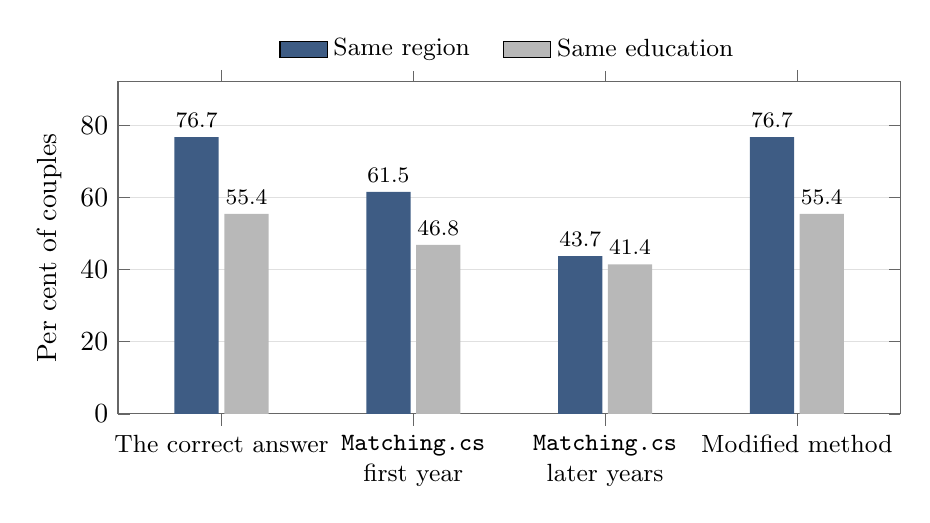
\begin{tikzpicture}
\begin{axis}[
  ybar, area legend, bar width=16pt, width=0.95\textwidth, height=5.8cm,
  ymin=0, ymax=92, enlarge x limits=0.18,
  ylabel={Per cent of couples},
  symbolic x coords={a,b,c,d}, xtick=data,
  xticklabels={{The correct answer},{\texttt{Matching.cs}\\first year},{\texttt{Matching.cs}\\later years},{Modified method}},
  x tick label style={align=center, font=\small},
  ymajorgrids, grid style={black!12}, axis line style={black!60}, tick style={black!60},
  nodes near coords,
  nodes near coords style={font=\footnotesize, /pgf/number format/.cd, fixed, fixed zerofill, precision=1},
  legend style={at={(0.5,1.03)}, anchor=south, legend columns=2, draw=none, font=\small, /tikz/every even column/.append style={column sep=1em}},
]
\addplot[fill=accent!85, draw=none] coordinates {(a,76.7) (b,61.5) (c,43.7) (d,76.7)};
\addplot[fill=black!28, draw=none] coordinates {(a,55.4) (b,46.8) (c,41.4) (d,55.4)};
\legend{Same region, Same education}
\end{axis}
\end{tikzpicture}
\caption{Share of couples in which the man and the woman live in the same region and have the same
education. Factor 1.3, average over 10 pools. The modified method is changes 0--3 with systematic,
sorted selection.}
\label{fig:nymetode}
\end{figure}

\begin{itemize}
\item \textbf{The error in \kode{Reset()} has a large effect on this market.} In later years only
43.7 per cent of the couples are from the same region, against 61.5 in the first year and 76.7 in
the true model, and 42.4 per cent of the couples are misplaced. How large the effect is in the
model depends on its data (Section~\ref{sec:nyforbehold}).
\item \textbf{Change 3 gives almost the whole improvement.} When the couples are formed in one
pass, all key figures hit the true model, and $D_{\text{joint}}$ falls from 20.7 to 5.0 or lower.
That confirms the explanation in Section~\ref{sec:fortolkning}: the loss of sorting arose in the
pairing.
\item \textbf{Change 2 matters when the pool is scaled up.} Without it, 7.0 per cent of the couples
are misplaced instead of 1.8, and those who get a partner resemble the pool less well (4.2 against
1.4 per cent). With factor 1.0 the change makes no difference.
\item \textbf{Change 1 cannot be measured on the standard pool.} Two RAS passes give the same key
figures as a finished adjustment. It is different when the pool does not resemble the historical
data (Section~\ref{sec:andrepuljer}).
\item \textbf{Systematic selection is more precise than independent draws.} Both hit the key
figures, but the systematic selection has less random variation: 1.8--3.3 per cent of the couples
are misplaced against 5.0. All three figures are lower than the 8.8 per cent that one random
outcome of the reference table gives.
\end{itemize}

The figure 1.8 for the sorted selection is a best case. The sorting uses the same groups as
$D_{\text{joint}}$ (five-year age groups, education and region), so exactly that measure is hit
particularly well. The figure 3.3 for the code's order is without that advantage.

The deviation that remains is random and not systematic. If the couples from the 10 pools are added
together in one table, $D_{\text{joint}}$ for the modified method falls from 1.8 to 0.6 per cent,
as random deviations do when there are more couples. For \kode{Matching.cs} in the first year the
figure is almost unchanged, 23.8 per cent.

Figure~\ref{fig:nymetode} shows the two most important key figures.

\subsection{Speed}\label{sec:hastighed}

Table~\ref{tab:tid} shows the time in one call of the matching on the standard pool with changes
0--3. Change 4 is not included here.

\begin{table}[htb]
\centering
\caption{Time in one call of the matching in ms without change 4, the standard pool, median over 10
pools. The figures in parentheses are the part that goes to the RAS adjustment and to the pairing.
The rest goes to sorting the pool into types and computing the sums. \kode{Matching.cs} is
unchanged and therefore has no breakdown.}
\label{tab:tid}
\small
\begin{tabular}{@{}lrrr@{}}
\toprule
 & Factor 1.0 & Factor 1.05 & Factor 1.3 \\
\midrule
\kode{Matching.cs}, first year & 812 & 50 & 46 \\
\kode{Matching.cs}, later years & 806 & 41 & 44 \\
\midrule
\multicolumn{4}{@{}l}{\emph{Modified method, one round}} \\
\quad 2 RAS passes (without change 1) & 30 (12 + 7) & 32 (12 + 8) & 34 (12 + 7) \\
\quad at most 10 RAS passes & 42 (24 + 7) & 45 (27 + 7) & 47 (25 + 7) \\
\quad RAS until the sums match (52--54 passes) & 113 (95 + 7) & 110 (87 + 7) & 112 (90 + 7) \\
\midrule
\multicolumn{4}{@{}l}{\emph{Modified method with mop-up rounds}} \\
\quad at most 10 RAS passes per round & 152 (111 + 25) & 89 (50 + 13) & 74 (48 + 12) \\
\quad RAS until the sums match & 755 (709 + 26) & 297 (257 + 14) & 207 (179 + 12) \\
\quad Number of rounds (with at most 10 passes) & 5.0 & 2.4 & 2.0 \\
\bottomrule
\end{tabular}
\end{table}

\begin{itemize}
\item \textbf{With scale-up the modified method is as fast as \kode{Matching.cs} without mop-up
rounds and takes 1.5--2 times as long with them.} With factors 1.05 and 1.3 \kode{Matching.cs}
takes 41--50 ms. The modified method with at most 10 RAS passes takes 45--47 ms in one round and
74--89 ms with mop-up rounds. The difference is 28--48 ms per call.
\item \textbf{Without scale-up the modified method is a good 5 times faster.} With factor 1.0
\kode{Matching.cs} takes about 810 ms, because the pairing goes through the cells many times to
find the last couples. The modified method takes 152 ms with mop-up rounds and 42 ms without. The
same happens with factor 1.05 when there are fewer men than women in the pool
(Section~\ref{sec:andrepuljer}).
\item \textbf{The pairing in one pass takes 7--8 ms regardless of the factor.} The original pairing
takes 6 ms with factor 1.3 and 10 ms with factor 1.05, but about 550 ms with factor 1.0. The three
figures are measured in the variant with changes 0+1, which has the original pairing.
\item \textbf{RAS is the largest item in the modified method.} A pass costs about 1.5 ms, and to
that are added about 10 ms per adjustment for the work that does not depend on the number of
passes. Running RAS until the sums match requires 52--54 passes and costs 60--70 ms more per round
than a cap of 10. It gives no measurable improvement on the standard pool (Table~\ref{tab:trin})
and a small improvement when the pool deviates from the historical data (Table~\ref{tab:ras}).
Change 4 removes most of the time spent on RAS (Section~\ref{sec:hurtigras}).
\item \textbf{A mop-up round costs 25--35 ms.} It consists of a new RAS adjustment and a new
pairing. With factor 1.3 one extra round is needed. With factor 1.0 all five rounds are used.
\end{itemize}

The times are measured on the test PC. They vary from measurement to measurement, so differences of
less than 10 ms should not be given any weight: four variants that do almost the same work lie
between 105 and 112 ms with factors 1.05 and 1.3.

The times are lower than in Section~\ref{sec:fortolkning}, where the matching took 0.1 and a good
1 second. Those figures are from a single call, in which .NET also has to compile the code to
machine code. Here the median over 10 calls is used, so that time does not count.

\subsection{Number of couples}

Change 3 has a price. When a type runs out, the cell's couples are lost. That also happens in
\kode{Matching.cs}, but it goes through the cells again until the number has been reached. With one
pass the lost couples are missing at the end. Table~\ref{tab:antalpar} shows how large a part of
the target is reached.

\begin{table}[htb]
\centering
\caption{Couples formed in per cent of the target. The modified method is changes 0--3 with at most
10 RAS passes. The small pool and the pool with fewer men are described in
Section~\ref{sec:andrepuljer}.}
\label{tab:antalpar}
\begin{tabular}{@{}lrrr@{}}
\toprule
 & Factor 1.0 & Factor 1.05 & Factor 1.3 \\
\midrule
\multicolumn{4}{@{}l}{\emph{Standard pool (36,000 couples)}} \\
\kode{Matching.cs}, first year & 99.56 & 100.00 & 100.00 \\
Modified method, one round & 97.83 & 99.36 & 99.97 \\
Modified method with mop-up rounds & 99.98 & 100.00 & 100.00 \\
\midrule
\multicolumn{4}{@{}l}{\emph{Small pool (3,600 couples)}} \\
\kode{Matching.cs}, first year & 99.55 & 100.00 & 100.00 \\
Modified method, one round & 88.02 & 90.60 & 96.93 \\
Modified method with mop-up rounds & 99.87 & 100.00 & 100.00 \\
\midrule
\multicolumn{4}{@{}l}{\emph{10 per cent fewer men than women}} \\
Highest possible (all men get a partner) & 94.74 & 99.48 & 100.00 \\
\kode{Matching.cs}, first year & 94.74 & 99.48 & 100.00 \\
Modified method, one round & 93.54 & 98.23 & 99.97 \\
Modified method with mop-up rounds & 94.73 & 99.47 & 100.00 \\
\bottomrule
\end{tabular}
\end{table}

In the standard pool 0.03 per cent of the couples are missing with factor 1.3 and 2.2 per cent with
factor 1.0. In the small pool, where there are few persons of each type, 3--12 per cent are
missing. Without mop-up rounds, change 3 is therefore not usable when the pool is small relative to
the number of types. With mop-up rounds the target is reached in all cases where it can be reached,
and the composition of the couples is unchanged (Tables~\ref{tab:trin} and~\ref{tab:andrepuljer}).

In the pool with fewer men, at most 94.74 and 99.48 per cent of the target can be reached with
factors 1.0 and 1.05, because the men run out. The shifted pool in Section~\ref{sec:andrepuljer}
gives the same figures as the standard pool: 97.5--99.95 per cent in one round and 99.97--100 per
cent with mop-up rounds.

\subsection{Other pools}\label{sec:andrepuljer}

The standard pool resembles the historical data and has equal numbers of men and women. Three other
pools test whether the results hold when that is not the case:

\begin{itemize}
\item \textbf{Small pool.} The pool is one tenth of the size, and 3,600 couples are to be formed.
There are few persons of each type: on average 11 with factor 1.3 and 9 with factor 1.0. 10 pools
per factor.
\item \textbf{Fewer men.} 10 per cent of the men in the pool have been removed at random. 5 pools
per factor.
\item \textbf{Shifted pool.} The probability of entering the pool rises with age and education. It
is half as large as in the standard pool for 20-year-olds and for the lowest level of education and
one and a half times as large for 54-year-olds and for the highest level. The pool thus has more
older people and more people with a long education than the historical data. 5 pools per factor.
\end{itemize}

The yardstick is the reference SBAM, that is, a correctly executed SBAM on the same pool. The true
model cannot be used in the shifted pool, because it is computed for a population with a different
composition. Table~\ref{tab:andrepuljer} shows the results with factor 1.3.

\begin{table}[htb]
\centering
\caption{Other pools, factor 1.3. The modified method is changes 0--3 with at most 10 RAS passes
and mop-up rounds, without change 4. $D_{\text{joint}}$ is relative to the reference SBAM. Time is
the median in ms.}
\label{tab:andrepuljer}
\small
\begin{tabular}{@{}lrrrrrr@{}}
\toprule
 & \multicolumn{2}{c}{Age gap} & \multicolumn{2}{c}{Same} & & \\
\cmidrule(lr){2-3}\cmidrule(lr){4-5}
 & mean & s.d. & edu. & reg. & $D_{\text{joint}}$ & Time \\
\midrule
\multicolumn{7}{@{}l}{\emph{Small pool}} \\
Reference SBAM (the correct answer) & 1.86 & 3.29 & 55.2 & 76.4 & 0.00 & -- \\
Reference SBAM, one draw & 1.85 & 3.31 & 55.0 & 76.2 & 25.84 & -- \\
\kode{Matching.cs}, first year & 1.88 & 3.32 & 53.3 & 75.1 & 24.89 & 26 \\
\kode{Matching.cs}, later years & 1.84 & 4.32 & 41.8 & 41.8 & 50.29 & 27 \\
Modified method & 1.87 & 3.26 & 55.2 & 76.6 & 13.99 & 66 \\
\midrule
\multicolumn{7}{@{}l}{\emph{Fewer men}} \\
Reference SBAM (the correct answer) & 1.84 & 3.28 & 55.4 & 76.7 & 0.00 & -- \\
Reference SBAM, one draw & 1.86 & 3.27 & 55.5 & 77.0 & 9.08 & -- \\
\kode{Matching.cs}, first year & 1.76 & 3.88 & 46.7 & 61.5 & 24.72 & 44 \\
\kode{Matching.cs}, later years & 1.80 & 4.52 & 41.3 & 43.4 & 42.37 & 46 \\
Modified method & 1.85 & 3.28 & 55.4 & 76.7 & 1.93 & 72 \\
\midrule
\multicolumn{7}{@{}l}{\emph{Shifted pool}} \\
Reference SBAM (the correct answer) & 1.75 & 3.50 & 58.6 & 76.7 & 0.00 & -- \\
Reference SBAM, one draw & 1.75 & 3.50 & 58.7 & 76.9 & 9.68 & -- \\
\kode{Matching.cs}, first year & 1.86 & 4.12 & 50.0 & 62.9 & 23.94 & 44 \\
\kode{Matching.cs}, later years & 1.84 & 4.73 & 45.0 & 44.6 & 41.51 & 43 \\
Modified method & 1.79 & 3.51 & 58.6 & 76.7 & 2.31 & 70 \\
\bottomrule
\end{tabular}
\end{table}

\begin{itemize}
\item \textbf{The modified method hits the correct answer in all three pools.} The shares with the
same education and region deviate by at most 0.2 percentage points from the reference SBAM, and
$D_{\text{joint}}$ is below what chance alone gives.
\item \textbf{In the small pool \kode{Matching.cs} is almost right in the first year.} The shares
are 53.3 and 75.1 per cent against 55.2 and 76.4, and $D_{\text{joint}}$ is at the level of chance.
The explanation is presumably that almost no cells are to give more than one couple in a small
pool. The first pass then forms almost all couples, and in that pass each cell has only one draw
(Section~\ref{sec:fortolkning}). The number of passes has not been measured. The bias in
\kode{Matching.cs} is thus largest in large pools. The error in \kode{Reset()}, by contrast, comes
through in full: 41.8 per cent from the same region in later years.
\item \textbf{With fewer men the age gap becomes too small in \kode{Matching.cs}.} It is 1.76
years against 1.84 in the reference SBAM. The modified method gives 1.85. Without change 2, RAS
cannot make the sums match in this pool, because the men's and the women's sums differ. The
adjustment then stops after about four passes.
\item \textbf{In the shifted pool the age gap is 1.79 years against 1.75 in the reference SBAM.}
\kode{Matching.cs} gives 1.86. The deviation of 0.04 years is due to the cap on RAS passes
(Table~\ref{tab:ras}).
\end{itemize}

With factors 1.0 and 1.05 all men in the pool with fewer men are to get a partner. Two things are
worth noting here. \kode{Matching.cs} takes 920 and 842 ms against 157 and 149 ms for the modified
method. And the mop-up rounds move the modified method a little away from the reference SBAM: the
age gap becomes 1.91--1.92 years against 1.85--1.86, and the standard deviation 3.31--3.32 against
3.28. The last men have to take the women who are left. \kode{Matching.cs} is further away, with
1.67 years and 3.63--3.64.

Table~\ref{tab:ras} shows the importance of the number of RAS passes.

\begin{table}[htb]
\centering
\caption{The importance of the number of RAS passes. Changes 0, 2 and 3 in one round, without
change 4, factor 1.3. $D_{\text{edu}}$ and $D_{\text{joint}}$ are relative to the reference SBAM. In
the last line for each pool RAS runs until the sums match.}
\label{tab:ras}
\small
\begin{tabular}{@{}lrrrrr@{}}
\toprule
 & RAS & RAS time, & Age & & \\
 & passes & ms & gap & $D_{\text{edu}}$ & $D_{\text{joint}}$ \\
\midrule
\multicolumn{6}{@{}l}{\emph{Standard pool (reference SBAM: 1.85 years)}} \\
As \kode{Matching.cs} & 2 & 12 & 1.87 & 0.03 & 1.94 \\
Cap of 10 & 10 & 25 & 1.86 & 0.02 & 1.83 \\
Until the sums match & 54 & 90 & 1.85 & 0.02 & 1.82 \\
\midrule
\multicolumn{6}{@{}l}{\emph{Shifted pool (reference SBAM: 1.75 years)}} \\
As \kode{Matching.cs} & 2 & 13 & 1.87 & 0.37 & 2.92 \\
Cap of 10 & 10 & 26 & 1.79 & 0.05 & 2.30 \\
Until the sums match & 67 & 109 & 1.75 & 0.03 & 2.17 \\
\bottomrule
\end{tabular}
\end{table}

In the standard pool two passes are enough. In the shifted pool they are not: the age gap becomes
1.87 years, which is close to the 1.88 years in the true model behind the historical data, and not
the 1.75 that fits the pool. In other words, the table does not get adjusted to the pool in time.
Ten passes remove most of the deviation and cost 14 ms. The rest requires 67 passes and 83 ms more.
The cap is a setting and can be set higher if the pools in the model deviate more from the
historical data than here. With change 4 all 67 passes cost 4 ms, and the cap can be dispensed with
(Section~\ref{sec:hurtigras}).

The test has also been run with types divided by municipality (3 pools). It gives the same picture
as with provinces. The modified method takes 81 ms against 53 ms for \kode{Matching.cs} with
factor 1.3 and 174 against 788 ms with factor 1.0.

\subsection{Change 4: The same table is computed faster}\label{sec:hurtigras}

Section~\ref{sec:hastighed} showed that the RAS adjustment is the largest item in the modified
method. With mop-up rounds and at most 10 passes, 48 of 74 ms go to RAS with factor 1.3 and 111 of
152 ms with factor 1.0. Change 4 computes the same adjusted table in a faster way. Only the method
of computation is changed. Changes 0--3 are the same as before.

\subsubsection*{Where the time goes}

The RAS adjustment is in \kode{RASMatrix.cs}, which both \kode{Matching.cs} and the modified method
use. Three things make it slow:

\begin{itemize}
\item \textbf{Each cell is a separate object.} The cells of a row are linked in a chain in which
each cell points to the next, and the same holds for the columns. The program has to follow the
chain from cell to cell. That is slower than reading numbers that lie in sequence in memory.
\item \textbf{Each pass goes through all cells four times.} The rows are summed, the cells of the
rows are multiplied by a factor, and then the same is done for the columns. The table has 72,908
cells, because each of the 36,454 cells with data appears twice (Section~\ref{sec:sbam}).
\item \textbf{Each call has a fixed amount of work.} After the last pass all cells are sorted, so
that the two mirror images of a cell can be added together. Afterwards all cells have to be reset
to the starting point.
\end{itemize}

\subsubsection*{The change}

The change consists of three techniques, 4a--4c, which can be switched on separately.

\textbf{4a: The computation is done on factors instead of cells.} RAS does only one thing:
multiplies a whole row or a whole column by a number. The adjusted cell is therefore always the
historical value times a factor for the row and a factor for the column. In the example in
Section~\ref{sec:sbam} the factors can be 0.551 for man 1 and 1.443 for woman 2, and the cell
becomes $20\cdot 0.551\cdot 1.443=15.9$. It is therefore enough to compute on the factors, two
numbers per type, and leave the historical values untouched. That saves time in four places:

\begin{itemize}
\item The historical values lie in one long sequence of numbers, row by row, without chains.
\item A pass reads the cells twice and does not write to them.
\item Which cells are mirror images of each other is found once at start-up and not by a sort in
each call.
\item The table does not have to be reset after the call. The error behind change 0 can therefore
not arise.
\end{itemize}

Pass by pass, 4a gives the same figures as \kode{RASMatrix.cs}, apart from rounding in the last
decimal.

\textbf{4b: One factor per type.} In the code's table men and women are in the same list of types,
and each couple is in two cells that are mirror images. Rows and columns are to match the same
sums, namely the number of persons of each type. A type can then have the same factor as row and as
column, and one factor per type is enough. The types are taken one at a time, and the type's factor
is set so that the type's sum matches, given the current factors of the other types. A pass reads
the cells once.

Without same-sex couples, each step is an ordinary RAS scaling of one row or one column in the
table with men in the rows and women in the columns. Only the order is different from 4a. The
result is therefore the same when the adjustment runs until the sums match, but not pass by pass. A
cell with two persons of the same type can only occur with same-sex couples. It gives a quadratic
equation in the type's factor, which is solved directly.

\textbf{4c: Only types with persons in the pool.} A type without persons in the pool has the sum 0,
and all its cells become 0. The computation is therefore done only on types with persons in the
pool and on cells between two such types, and only those cells are passed on to the pairing. The
technique is effective especially in the mop-up rounds, where few types are left. In the model the
table has 28,050 types, and the pool hardly contains all of them. There the technique may also
matter in the first round. That has not been measured.

\subsubsection*{Check that the table is the same}

\begin{itemize}
\item \textbf{4a forms exactly the same couples.} The modified method has been run with and without
4a on the same pools with the same seed. The couples are the same, couple by couple, in all 96
runs: 30 on the standard pool, 30 on the small pool, 15 with fewer men, 15 on the shifted pool and
6 with types by municipality.
\item \textbf{4b and 4c do not give the same couples, but the same composition.} With a cap of 10
passes the table from 4b is slightly different from the table from 4a. With 4c the pairing gets
fewer cells and therefore uses the random numbers differently. The key figures are unchanged. On
the standard pool with factor 1.3, 55.4 per cent of the couples have the same education, 76.7 per
cent are from the same region, and $D_{\text{joint}}$ is 1.83--1.84 per cent both with and without
change 4.
\item \textbf{The RAS part has been checked separately.} The methods of computation have been
compared on 20 random symmetric tables with 30--59 types, which also have cells with two of the
same type. All have been run until the sums match. The largest relative deviation in a cell from
\kode{RASMatrix.cs} is $3\cdot10^{-13}$ with 4a and $6\cdot10^{-13}$ with 4b.
\end{itemize}

\subsubsection*{Speed}

Table~\ref{tab:hurtig} shows the time on the standard pool when the techniques are switched on one
by one.

\begin{table}[htb]
\centering
\caption{Time in one call of the matching in ms with and without change 4, the standard pool,
median over 10 pools. All lines except \kode{Matching.cs} have changes 0--3 with systematic, sorted
selection. The figures in parentheses are the part that goes to the RAS adjustment and to the
pairing.}
\label{tab:hurtig}
\small
\begin{tabular}{@{}lrrr@{}}
\toprule
 & Factor 1.0 & Factor 1.05 & Factor 1.3 \\
\midrule
\kode{Matching.cs}, first year & 812 & 50 & 46 \\
\kode{Matching.cs}, later years & 806 & 41 & 44 \\
\midrule
\multicolumn{4}{@{}l}{\emph{At most 10 RAS passes per round, with mop-up rounds}} \\
\quad without change 4 & 152 (111.0 + 24.9) & 89 (50.2 + 13.1) & 74 (48.3 + 12.2) \\
\quad with 4a & 38 (6.4 + 20.4) & 25 (3.6 + 10.8) & 26 (2.5 + 10.6) \\
\quad with 4a and 4b & 36 (4.6 + 21.6) & 24 (2.0 + 10.7) & 25 (1.7 + 11.7) \\
\quad with 4a, 4b and 4c & 22 (2.1 + 8.1) & 24 (2.5 + 9.8) & 24 (2.1 + 10.8) \\
\midrule
\multicolumn{4}{@{}l}{\emph{RAS until the sums match, with mop-up rounds}} \\
\quad without change 4 & 755 (708.7 + 26.3) & 297 (256.7 + 13.9) & 207 (178.5 + 11.9) \\
\quad with 4a, 4b and 4c & 26 (5.7 + 8.6) & 31 (10.0 + 11.4) & 32 (8.1 + 10.5) \\
\midrule
\multicolumn{4}{@{}l}{\emph{At most 10 RAS passes, one round}} \\
\quad without change 4 & 42 (23.7 + 7.1) & 45 (27.0 + 7.1) & 47 (25.0 + 7.1) \\
\quad with 4a, 4b and 4c & 17 (1.1 + 7.1) & 17 (1.1 + 6.6) & 21 (1.1 + 7.8) \\
\midrule
\multicolumn{4}{@{}l}{\emph{RAS until the sums match (52--55 passes), one round}} \\
\quad without change 4 & 113 (95.4 + 7.3) & 110 (86.7 + 7.2) & 112 (89.9 + 7.3) \\
\quad with 4a, 4b and 4c & 21 (3.3 + 7.2) & 21 (3.4 + 6.7) & 22 (3.4 + 7.0) \\
\bottomrule
\end{tabular}
\end{table}

\begin{itemize}
\item \textbf{The RAS time falls to one twentieth or less.} With at most 10 passes per round it
falls from 48--111 ms to 2.1--2.5 ms. When RAS runs until the sums match, it falls from 179--709 ms
to 6--10 ms.
\item \textbf{4a gives almost the whole gain.} The RAS time falls from 111 to 6.4 ms with factor
1.0 and from 48 to 2.5 ms with factor 1.3. 4b removes between a quarter and just under half of
what is left.
\item \textbf{4c is effective when there are many mop-up rounds.} With factor 1.0 and five rounds
the RAS time falls from 4.6 to 2.1 ms and the pairing from 22 to 8 ms, because the pairing in the
last rounds gets only the few cells that are left. With two rounds there is no measurable
difference.
\item \textbf{A pass costs 0.05 ms against 1.5 ms before.} In one round 10 passes cost 1.1 ms and
52--55 passes 3.3--3.4 ms. The fixed work per adjustment thus costs about 0.6 ms against about
10 ms before.
\item \textbf{The cap of 10 passes is superfluous.} Running RAS until the sums match costs 4--8 ms
more per call than a cap of 10: 26, 31 and 32 ms against 22, 24 and 24. Without change 4 it costs
133--603 ms more.
\item \textbf{The modified method is now at least as fast as \kode{Matching.cs} with scale-up and
about 30 times faster without.} With RAS until the sums match and mop-up rounds it takes 26--32 ms.
\kode{Matching.cs} takes 41--50 ms with scale-up and about 810 ms without.
\item \textbf{RAS is no longer the largest item.} Of the 32 ms with factor 1.3, 8 go to RAS and 11
to the pairing. The remaining 13 ms or so go to sorting the pool into types and computing the sums.
That part has not been changed.
\end{itemize}

As in Section~\ref{sec:hastighed}, the total times vary by a few ms from measurement to
measurement.

\subsubsection*{All pools}

When RAS is cheap, it can run until the sums match in all rounds. Table~\ref{tab:hurtigpuljer}
compares that method with the method from Table~\ref{tab:andrepuljer}, which has a cap of 10 passes
and does not use change 4.

\begin{table}[htb]
\centering
\caption{The modified method with and without change 4, factor 1.3. Both have changes 0--3 and
mop-up rounds. $D_{\text{joint}}$ is relative to the reference SBAM. Time is the median in ms.}
\label{tab:hurtigpuljer}
\small
\begin{tabular}{@{}lrrrrrr@{}}
\toprule
 & \multicolumn{2}{c}{Age gap} & \multicolumn{2}{c}{Same} & & \\
\cmidrule(lr){2-3}\cmidrule(lr){4-5}
 & mean & s.d. & edu. & reg. & $D_{\text{joint}}$ & Time \\
\midrule
\multicolumn{7}{@{}l}{\emph{Standard pool}} \\
Reference SBAM (the correct answer) & 1.85 & 3.28 & 55.4 & 76.7 & 0.00 & -- \\
Cap of 10 passes, without change 4 & 1.86 & 3.28 & 55.4 & 76.7 & 1.84 & 74 \\
Until the sums match, with change 4 & 1.85 & 3.28 & 55.4 & 76.7 & 1.83 & 32 \\
\midrule
\multicolumn{7}{@{}l}{\emph{Small pool}} \\
Reference SBAM (the correct answer) & 1.86 & 3.29 & 55.2 & 76.4 & 0.00 & -- \\
Cap of 10 passes, without change 4 & 1.87 & 3.26 & 55.2 & 76.6 & 13.99 & 66 \\
Until the sums match, with change 4 & 1.87 & 3.25 & 55.2 & 76.6 & 13.78 & 19 \\
\midrule
\multicolumn{7}{@{}l}{\emph{Fewer men}} \\
Reference SBAM (the correct answer) & 1.84 & 3.28 & 55.4 & 76.7 & 0.00 & -- \\
Cap of 10 passes, without change 4 & 1.85 & 3.28 & 55.4 & 76.7 & 1.93 & 72 \\
Until the sums match, with change 4 & 1.84 & 3.28 & 55.4 & 76.7 & 1.92 & 31 \\
\midrule
\multicolumn{7}{@{}l}{\emph{Shifted pool}} \\
Reference SBAM (the correct answer) & 1.75 & 3.50 & 58.6 & 76.7 & 0.00 & -- \\
Cap of 10 passes, without change 4 & 1.79 & 3.51 & 58.6 & 76.7 & 2.31 & 70 \\
Until the sums match, with change 4 & 1.75 & 3.50 & 58.6 & 76.7 & 2.18 & 30 \\
\bottomrule
\end{tabular}
\end{table}

Table~\ref{tab:hurtigtid} shows the time for all factors.

\begin{table}[htb]
\centering
\caption{Time in one call of the matching in ms, median over the pools. ``Modified'' is changes
0--4 with RAS until the sums match and mop-up rounds. \kode{Matching.cs} is the first year. Types
by municipality have not been run with factor 1.05.}
\label{tab:hurtigtid}
\small\setlength{\tabcolsep}{5pt}
\begin{tabular}{@{}lrrrrrr@{}}
\toprule
 & \multicolumn{2}{c}{Factor 1.0} & \multicolumn{2}{c}{Factor 1.05} & \multicolumn{2}{c}{Factor 1.3} \\
\cmidrule(lr){2-3}\cmidrule(lr){4-5}\cmidrule(l){6-7}
 & \kode{Matching.cs} & Modified & \kode{Matching.cs} & Modified & \kode{Matching.cs} & Modified \\
\midrule
Standard pool & 812 & 26 & 50 & 31 & 46 & 32 \\
Small pool & 965 & 16 & 27 & 19 & 26 & 19 \\
Fewer men & 920 & 32 & 842 & 32 & 44 & 31 \\
Shifted pool & 923 & 24 & 46 & 27 & 44 & 30 \\
Types by municipality & 788 & 28 & -- & -- & 53 & 36 \\
\bottomrule
\end{tabular}
\end{table}

\begin{itemize}
\item \textbf{The precision is the same or better.} In the standard pool, the small pool and the
pool with fewer men the figures are almost the same as with the cap. In the shifted pool the age
gap now hits the reference SBAM: 1.75 years against 1.79 with the cap (Table~\ref{tab:ras}).
\item \textbf{The modified method has the lowest time in all 14 cases.} It takes 16--36 ms per
call. \kode{Matching.cs} takes 26--53 ms when it finds the couples easily and 788--965 ms when it
does not. In the small pool with scale-up the difference is 7--8 ms and no larger than the
measurement uncertainty.
\item \textbf{The time depends only a little on the pool and the factor.} The longest time is a
good 2 times the shortest. For \kode{Matching.cs} the ratio is 37.
\end{itemize}

The times for \kode{Matching.cs} in later years are at the same level as in the first year.

\subsubsection*{An edge-case bug in \kode{RASMatrix.cs}}

The work on change 4 revealed a minor error in \kode{RASMatrix.cs}. When the cells are linked
together in rows and columns, the loop stops one cell too early (lines 102 and 128):

{\small
\begin{verbatim}
    for (int i = 0; i < n - 1; i++)
\end{verbatim}
}

The last cell is therefore only included if it is in the same row or column as the cell before it.
If the type with the highest number in the historical data has only one cell, it is treated as a
type without data. Its sum is set to 0, so the table gives the type no couples. The error has been
demonstrated on an example with three types. It can affect at most one type and has no importance
on the test market. The method of computation in change 4 does not have the error.

\subsection{Overall assessment and caveats}\label{sec:nyforbehold}

The method this section points to consists of four parts:

\begin{itemize}
\item changes 0, 2 and 3 with systematic, sorted selection,
\item change 1, where RAS runs until the sums match,
\item change 4 with all three techniques,
\item mop-up rounds.
\end{itemize}

In all the pools tested and for all three factors it forms at least 99.85 per cent of the couples
that can be formed, and hits the correct answer. The shares with the same education and region
deviate by at most 0.2 percentage points from the reference SBAM in the large pools and at most 0.6
in the small one, where chance alone gives deviations of the same size. The age gap deviates by at
most 0.07 years. The largest deviation is in the pool with fewer men, where the last men have to
take the women who are left (Section~\ref{sec:andrepuljer}). A call takes 16--36 ms against
26--965 ms for \kode{Matching.cs}.

Change 4 makes two trade-offs from the preceding sections superfluous:

\begin{itemize}
\item \textbf{The cap of 10 RAS passes.} Running RAS until the sums match costs 1--12 ms more per
call than a cap of 10 and removes the deviation the cap gives in the shifted pool.
\item \textbf{The mop-up rounds.} They cost 2--14 ms per call. Without them 0.03--0.04 per cent of
the couples are missing in the large pools with factor 1.3, about 1 per cent with factor 1.05 and
3--12 per cent in the small pool.
\end{itemize}

If change 4 is not used, the cap of 10 passes should be kept. A call then takes 66--81 ms with
factor 1.3. That is 26--40 ms more than \kode{Matching.cs}.

The caveats are:

\begin{itemize}
\item \textbf{The effect of the error in \kode{Reset()} in the model is not known.} The error means
that all cells count 1 from the second year. On the test market a cell with data contains on
average 5 historical couples, so much information is lost. If most cells in the model's data
contain only one couple, the loss is smaller. That can only be settled with the model's data.
\item \textbf{The running times apply to the test market.} The model's table has more cells and
more types. The time for RAS grows with the number of cells and passes, and the time for the
pairing with the number of cells and couples. The ratio between the methods and the gain from
change 4 may therefore be different in the model.
\item \textbf{Same-sex couples have not been tested.} The historical test data contain none, and
the code treats them separately. Change 2 scales men and women separately to the number of couples
and does not take same-sex couples into account. That must be clarified before the change is used
on the model's data. In change 4 the treatment of cells with two of the same type has only been
tested in the RAS part on random tables and not in the pairing.
\item \textbf{Change 4 requires a symmetric table.} The table in \kode{Matching.cs} is symmetric,
because each historical couple is entered in both mirror cells. The code checks this and stops with
an error if the table is not symmetric.
\item \textbf{Types without historical data have still not been dealt with.} Persons of a type that
is not found in the data get no partner, not even in the mop-up rounds. That is the next thing that
should be solved.
\item \textbf{The error in the age grouping has not been corrected} (Section~\ref{sec:forbehold}).
\item \textbf{One set of historical data.} The pools vary, but the historical data are the same in
all runs.
\item \textbf{The changes have not been put into the model.} They exist only in
\kode{Matching\_test.cs} and \kode{RASMatrix\_test.cs} in the test program.
\end{itemize}


\section{Limitations}\label{sec:forbehold}

The limitations in this section apply to the test of \kode{Matching.cs} in
Sections~\ref{sec:opstilling}--\ref{sec:fortolkning}. The caveats for the modified method are in
Section~\ref{sec:nyforbehold}.

\begin{itemize}
\item \textbf{Only the model's first year.} The matching is called once. From the second year the
code no longer uses the historical table, and the sorting is weaker (Section~\ref{sec:aendringer}).
\item \textbf{One run per setting.} There is one set of historical data and one seed. The
importance of chance has instead been assessed with the rows ``one draw'', and the deviations in
education and region are far above them. Section~\ref{sec:nymetode} uses 3--10 pools per setting
and gives the same picture.
\item \textbf{The age grouping has not been tested.} A reading of the code suggests an error when
it reads the historical data: the age is limited to 15--65 years, and then 1 is added, so the
oldest end up outside the age interval and are counted in a wrong type. The market has only
20--54-year-olds, so the test does not touch the error.
\item \textbf{Types without historical data have not been tested.} In the model there may be
persons in the pool whose type has never been seen in the data. RAS cannot give them a partner. In
the test all the types of the pool are found in the data (Section~\ref{sec:indlejring}).
\item \textbf{Only a small part of SMILE's types are in use.} The test uses 840 of 28,050 types and
one origin group. The running times therefore say nothing about the model.
\item \textbf{The same factor everywhere.} The model uses factors between 1.05 and 1.3 depending on
the municipality. The test uses one factor for all.
\item \textbf{The pool resembles the historical population.} The test says nothing about how the
code copes with a population with a different composition, for example more older people or more
men than women. Two such pools have been tried in Section~\ref{sec:andrepuljer}.
\item \textbf{The RAS table has been recomputed.} The code's RAS table has been computed in the
test program and not read from inside the code (Section~\ref{sec:fortolkning}).
\item \textbf{Only the matching has been tested.} What the model does with a new couple afterwards
(choice of dwelling, moving and formation of the new household) is switched off.
\item \textbf{The data period is different from the model's.} The model uses a variant of the code,
\kode{Matching2019}, which selects historical data for 2013--2017 and sets the factors. The test
uses the basic version, which selects 2008--2012. The algorithm is the same in the two.
\end{itemize}


\section{The test program}

The test program is in the folder \kode{CodeTest} and consists of four kinds of files:

\begin{description}[leftmargin=1.5em, style=nextline]
\item[\kode{Matching.cs}] A copy of the model's file. The original in the model folder
(\path{C:\psp\MS_SMILE_2026}) is untouched. At the top of the copy is \kode{\#define SBAM\_TEST}.
When that constant is defined, the parts that require the rest of the model are switched off:
writing of report files and everything that happens to a couple after it has been formed. Reading
of data, division into types, RAS and pairing are unchanged. If the constant is removed, the code
is the same as in the original.

\item[\kode{SmileFiles\textbackslash}] Copies of the 11 other model files that \kode{Matching.cs}
uses, among them \kode{RASMatrix.cs} with the RAS adjustment. Nine are unchanged. In
\kode{Dwelling.cs} and \kode{Mappings.cs} one method each is switched off with the same constant.

\item[\kode{Test\textbackslash}] The test's own code, which is not model code. \kode{Market.cs}
computes the artificial market. \kode{Program.cs} writes the historical data, forms the pool, runs
the matching and measures the result. \kode{TestStubs.cs} contains simple replacements for the
parts of the model that the code expects to be present, for example persons and households.
\kode{Sammenlign.cs} runs the comparison in Section~\ref{sec:nymetode}.

\item[\kode{Matching\_test.cs} and \kode{RASMatrix\_test.cs}] Copies of \kode{Matching.cs} and
\kode{RASMatrix.cs} with the changes from Section~\ref{sec:nymetode}. The changes are marked
\kode{//TEST0} to \kode{//TEST4} and can be switched on and off separately. With all of them
switched off, the code forms the same couples as \kode{Matching.cs}.
\end{description}

The program's printouts and command-line options are in Danish, and so are the comments in the
code taken over from the model. The test's own code and the changes are commented in English.

The program builds for .NET~8. The model is set to .NET~7, which is not installed on the machine.
The test is run from the folder \kode{CodeTest}:

{\small
\begin{verbatim}
dotnet run                    (factor 1.0, provinces)
dotnet run -- --scale 1.3     (factor 1.3)
dotnet run -- --kommune       (types by municipality)
dotnet run -- --seed 2        (another seed for pool and pairing)
\end{verbatim}
}

The historical data have a fixed seed and are the same in all runs. The pool and the pairing are
controlled by \kode{-{}-seed}. The run with \kode{-{}-seed 2} has not been made for this paper.

The comparison in Section~\ref{sec:nymetode} is run like this:

{\small
\begin{verbatim}
dotnet run -c Release -- --sammenlign --koersler 10
dotnet run -c Release -- --sammenlign --koersler 10 --pulje 0.1    (small pool)
dotnet run -c Release -- --sammenlign --koersler 5 --skaev 0.1     (fewer men)
dotnet run -c Release -- --sammenlign --koersler 5 --forskyd 0.5   (shifted pool)
dotnet run -c Release -- --sammenlign --koersler 3 --kommune --faktorer 1.0,1.3
\end{verbatim}
}

Each run computes factors 1.0, 1.05 and 1.3, unless otherwise specified with \kode{-{}-faktorer}.
The environment variable \kode{DOTNET\_TieredCompilation=0} was set when the times in the paper
were measured. It makes .NET compile the code fully optimised the first time,
so that all variants are measured on equal terms. Each run begins with the check of the RAS part on
random tables from Section~\ref{sec:hurtigras}.

The results are in \kode{CodeTest}:

\begin{center}
\begin{tabular}{@{}ll@{}}
\toprule
File & Contents \\
\midrule
\kode{output\textbackslash koersel\_scale\_1.0.txt} & Printout, factor 1.0 \\
\kode{output\textbackslash koersel\_scale\_1.3.txt} & Printout, factor 1.3 \\
\kode{output\textbackslash koersel\_kommune.txt} & Printout, types by municipality \\
\kode{output\textbackslash testMatching2\_*.txt} & The code's own counters for each run \\
\kode{output\textbackslash sammenligning*.txt} & Printouts from the comparison in Section~\ref{sec:nymetode} \\
\kode{data\textbackslash SBAM\_testdata\_enlige.txt} & Singles per type \\
\kode{data\textbackslash SBAM\_testdata\_nyePar\_2008\_2012.txt} & The historical couples \\
\bottomrule
\end{tabular}
\end{center}


\appendix
\section{The artificial marriage market}\label{app:parametre}

The market has been constructed for this test. It has been chosen so that the sorting has the
features known from real couples, and so that the correct answer can be computed. The appendix
describes the market in full, so that it can be recreated. The computation is in the file
\kode{Market.cs} in the test program. Below, $a$ is age, $e$ education and $r$ region, and $f$ is 1
for women and 0 for men.

\subsection{Types and population}

A type is a combination of age (20--54 years in one-year steps), education (levels 1--3, where 1 is
the lowest) and region (1--4). That gives $35\cdot3\cdot4=420$ types for each sex.

Each sex has 300,000 singles, distributed over types in proportion to
$w_{\text{age}}\cdot w_{\text{reg}}\cdot w_{\text{edu}}$:
\begin{align*}
w_{\text{age}} &= e^{-0.06\,(a-20)}+0.25, \qquad w_{\text{reg}} = (0.35,\ 0.25,\ 0.25,\ 0.15),\\
p_{\text{high}} &= \Lambda\bigl(-1.2+0.6f-0.02\,(a-20)+0.5\cdot[\text{region 1}]\bigr),\\
p_{\text{low}} &= (1-p_{\text{high}})\,\Lambda\bigl(-1.0-0.3f+0.02\,(a-20)-0.3\cdot[\text{region 1}]\bigr),
\end{align*}
where $\Lambda(z)=1/(1+e^{-z})$, and $[\text{region 1}]$ is 1 for region 1 and 0 for the others.
$w_{\text{edu}}$ is $p_{\text{low}}$ for the lowest education, $p_{\text{high}}$ for the highest and
$1-p_{\text{high}}-p_{\text{low}}$ for the middle one. The weights mean:

\begin{itemize}
\item $w_{\text{age}}$: most singles are young. There are a good three times as many 20-year-olds
as 54-year-olds.
\item $w_{\text{reg}}$: region 1 is the largest with 35 per cent of the singles, and region 4 the
smallest.
\item $p_{\text{high}}$ and $p_{\text{low}}$: the women are better educated than the men, the young
better than the old, and region 1 better than the other regions.
\end{itemize}

The number of singles of each type is rounded to whole persons. That gives 299,997 men and 300,003
women. The number of single men of type $x$ is called $M^A_x$ and the number of single women of
type $y$ is called $M^B_y$.

\subsection{The model of pairing}

The true couple table has been computed with Choo and Siow's (2006) model of the marriage market.
In the model each single chooses between remaining single and forming a couple with a partner of
one of the 420 types. The gain from a choice consists of a part that is common to all of the same
type and a random part that is the person's own taste. Everyone chooses what is best for
themselves. The market is in equilibrium when the number of men of type $x$ who choose a woman of
type $y$ equals the number of women of type $y$ who choose a man of type $x$. In equilibrium the
number of couples is
\[
\mu_{xy}=\sqrt{\mu_{x0}\,\mu_{0y}}\;\exp(\Phi_{xy}/2) .
\]
Here $\mu_{xy}$ is the number of couples between men of type $x$ and women of type $y$, $\mu_{x0}$
and $\mu_{0y}$ are the numbers of men and women of the two types who remain single, and $\Phi_{xy}$
is the joint gain the two have from forming a couple rather than remaining single. All singles
either form a couple or remain single:
\[
\mu_{x0}+\sum_y\mu_{xy}=M^A_x, \qquad \mu_{0y}+\sum_x\mu_{xy}=M^B_y .
\]
The three equations determine the couple table when the population and the gain are given, and they
have exactly one solution (Decker et al., 2013).

\subsection{The gain}

The gain for a man of type $x$ and a woman of type $y$ is
\[
\frac{\Phi_{xy}}{2}=\kappa+h_A(a_x)+h_B(a_y)-\frac{(a_x-a_y-2)^2}{2\,\tau(\bar a_{xy})^2}
+\rho^E_{e_xe_y}+\rho^R_{r_xr_y},
\]
where $\bar a_{xy}=(a_x+a_y)/2$ is the couple's average age. The terms are explained in
Section~\ref{sec:opstilling}. They have the values
\begin{align*}
h_A(a) &= -0.035\,(a-20), \qquad h_B(a) = -0.045\,(a-20), \qquad \tau(\bar a) = 2+0.12\,(\bar a-20),\\
\rho^E &= \begin{pmatrix} 0.8 & 0 & -0.9\\ 0 & 0.5 & 0\\ -0.9 & 0 & 0.9 \end{pmatrix},
\qquad
\rho^R = \begin{pmatrix} 0 & -1.5 & -2.6 & -2.6\\ -1.5 & 0 & -2.6 & -2.6\\ -2.6 & -2.6 & 0 & -2.6\\ -2.6 & -2.6 & -2.6 & 0 \end{pmatrix}.
\end{align*}
The rows of $\rho^E$ and $\rho^R$ are the man's education and region, and the columns are the
woman's. The constant $\kappa$ is determined together with the solution.

\subsection{Computation of the true couple table}

Let $K_{xy}=\exp(\Phi_{xy}/2)$, $\alpha_x=\sqrt{\mu_{x0}}$ and $\beta_y=\sqrt{\mu_{0y}}$. Then
$\mu_{xy}=\alpha_x\beta_yK_{xy}$, and the equation for the men of type $x$ becomes a quadratic
equation in $\alpha_x$:
\[
\alpha_x^2+\alpha_x S_x=M^A_x, \qquad S_x=\sum_yK_{xy}\beta_y,
\qquad\text{with the solution}\qquad
\alpha_x=\sqrt{M^A_x+S_x^2/4}-S_x/2 .
\]
The equation for the women of type $y$ has the same form with $S_y=\sum_xK_{xy}\alpha_x$ and
$M^B_y$. The iterative method of Galichon and Salanié (2022) solves the two sets of equations
alternately: first all $\alpha_x$ are computed from the current $\beta_y$, then all $\beta_y$ from
the new $\alpha_x$. The starting values are $\alpha_x=\sqrt{M^A_x}$ and $\beta_y=\sqrt{M^B_y}$, and
the steps are repeated until no value changes by more than a relative deviation of $10^{-13}$.

The constant $\kappa$ has been set so that 12 per cent of the single men find a partner in a year.
It has been found by solving the model for different values of $\kappa$ between $-15$ and 0 until
the share matches. That gives $\kappa=-4.5616$ and 36,000 couples per year. In the final solution
no type's sum deviates by more than $9\cdot10^{-13}$ persons from the number of singles of the
type.

The key figures of the true couple table are in Table~\ref{tab:marked}. How the historical data and
the pool are drawn from the table is described in Section~\ref{sec:opstilling}.


\needspace{14\baselineskip}
\section*{References}
\markboth{References}{}

\small
\begin{description}[leftmargin=1.5em, itemsep=0pt, font=\normalfont]
\item Choo, E. and A. Siow (2006). Who marries whom and why. \emph{Journal of Political Economy},
114(1), 175--201.
\item Decker, C., E. H. Lieb, R. J. McCann and B. K. Stephens (2013). Unique equilibria and
substitution effects in a stochastic model of the marriage market. \emph{Journal of Economic
Theory}, 148(2), 778--792.
\item Duncan, O. D. and B. Duncan (1955). A methodological analysis of segregation indexes.
\emph{American Sociological Review}, 20(2), 210--217.
\item Galichon, A. and B. Salanié (2022). Cupid's invisible hand: Social surplus and identification
in matching models. \emph{The Review of Economic Studies}, 89(5), 2600--2629.
\item Stephensen, P. and T. Markeprand (2013). SBAM: An algorithm for pair matching. DREAM Working
Paper 2013:3.
\end{description}

\end{document}
